\chapter{Alkena dan Alkuna: Adisi Elektrofilik}\label{ch:b1:electrophilic-additions}

Kocoklah sebuah alkena dengan air brom yang berwarna jingga, maka warnanya
lenyap dalam beberapa detik: uji tertua untuk ikatan rangkap dua
karbon--karbon. Di balik uji itu ada sebuah mekanisme. Elektron $\pi$
ikatan rangkap dua, yang terikat kurang kuat daripada elektron $\sigma$
dan terpapar di atas dan di bawah bidang molekul, menyerang pereaksi yang
miskin elektron; kation yang terbentuk lalu menangkap sebuah \omterm{def:b1:electronic-effects:nucleophile}{nukleofil}.
Dua tahap yang sama itu mengadisikan hidrogen halida, air, dan halogen
pada alkena, menentukan karbon mana yang menerima bagian mana dari
pereaksi, dan menetapkan stereokimia produknya. Bab ini mengembangkan
kedua tahap itu, beserta aturan yang ditarik seorang kimiawan abad
kesembilan belas dari pengamatan dan \omterm{def:b1:electronic-effects:intermediates}{karbokation} yang menjelaskannya.

\begin{recall}
\omterm{def:b1:electronic-effects:intermediates}{Karbokation}, kestabilannya, dan \omterm{def:b1:electronic-effects:curly-arrow}{panah lengkung} (\cref{ch:b1:electronic-effects});
postulat Hammond (\cref{prop:b1:elementary-steps:hammond}); deskriptor
$Z$/$E$, \cip{R}/\cip{S}, \omterm{def:b1:stereochemistry-in-depth:enantiomers}{senyawa meso}, dan \omterm{def:b1:stereochemistry-in-depth:enantiomers}{campuran rasemat}
(\cref{ch:b1:stereochemistry-in-depth}). Jilid sekolah (kelas 12) telah
mendaftar adisi-adisi alkena tanpa mekanismenya.
\end{recall}

\section{Ikatan \texorpdfstring{$\pi$}{pi} sebagai nukleofil}

\begin{definition}[Adisi elektrofilik]\label{def:b1:electrophilic-additions:electrophilic-addition}
\emph{Adisi elektrofilik}\index{adisi elektrofilik} pada ikatan rangkap
adalah adisi yang tahap pertamanya berupa serangan elektron $\pi$ pada
sebuah \omterm{def:b1:electronic-effects:nucleophile}{elektrofil} E: terbentuk sebuah kation, yang lalu menangkap
\omterm{def:b1:electronic-effects:nucleophile}{nukleofil} Nu, sehingga E dan Nu akhirnya berada pada kedua karbon bekas
ikatan rangkap dua itu.
\end{definition}

Ikatan $\pi$ adalah yang lebih lemah di antara kedua ikatan C=C (\cref{ch:b1:lewis-resonance-vsepr}),
dan elektronnya terletak jauh dari inti, di atas dan di bawah bidang:
alkena adalah \omterm{def:b1:electronic-effects:nucleophile}{nukleofil}, dan bereaksi dengan asam, halogen, dan \omterm{def:b1:electronic-effects:nucleophile}{elektrofil}
lain yang membiarkan alkana jenuh tetap utuh.

\section{Adisi hidrogen halida: aturan Markovnikov}

\begin{omfigure}
\setchemfig{atom sep=2.1em}
\schemestart
\chemfig{H_3C-[:30]@{c2}CH=[@{pi},,,,]@{c1}CH_2}
\+
\chemfig{@{h}H-[@{hb}]@{br}Br}
\arrow{->}
\chemfig{H_3C-[:30]CH^{+}-[:-30]CH_3}
\+
\chemfig{Br^{-}}
\arrow{->}
\chemfig{H_3C-[:30]CH(-[2]Br)-[:-30]CH_3}
\schemestop
\chemmove{\draw[->, thick, shorten <=2pt, shorten >=2pt](pi) .. controls +(90:7mm) and +(110:7mm) .. (h);
          \draw[->, thick, shorten <=2pt, shorten >=2pt](hb) .. controls +(-90:5mm) and +(-90:5mm) .. (br);}

{\small Adisi hidrogen bromida pada propena. Pasangan $\pi$ mengambil
proton, ke karbon ujung, sehingga terbentuk \omterm{def:b1:electronic-effects:intermediates}{karbokation} sekunder; ion
bromida beradisi padanya: 2-bromopropana.}
\end{omfigure}

\begin{proposition}[Aturan Markovnikov]\label{prop:b1:electrophilic-additions:markovnikov}
Pada adisi HX pada alkena yang tidak simetris, hidrogen menuju karbon
ikatan rangkap dua yang telah membawa lebih banyak hidrogen
(\emph{aturan Markovnikov}\index{aturan Markovnikov}). Dalam bentuk
modern: \omterm{def:b1:electronic-effects:nucleophile}{elektrofil} beradisi sedemikian rupa sehingga menghasilkan
\omterm{def:b1:electronic-effects:intermediates}{karbokation} yang lebih stabil.
\end{proposition}

\begin{proof}
Perpindahan proton adalah \omterm{def:b1:elementary-steps:rds}{tahap penentu laju}, endoterm, dan berakhir
pada sebuah \omterm{def:b1:electronic-effects:intermediates}{karbokation}. Menurut postulat Hammond
(\cref{prop:b1:elementary-steps:hammond}) \omterm{def:b1:elementary-steps:energy-profile}{keadaan transisinya} menyerupai
\omterm{def:b1:electronic-effects:intermediates}{karbokation} itu, sehingga jalan menuju \omterm{def:b1:electronic-effects:intermediates}{karbokation} yang lebih stabil
mempunyai sawar yang lebih rendah dan jauh lebih cepat. Menempatkan
proton pada karbon yang membawa lebih banyak hidrogen meninggalkan muatan
pada karbon yang membawa lebih banyak gugus alkil, yaitu kation yang
lebih stabil (\cref{prop:b1:electronic-effects:carbocation-order}).
\end{proof}

\begin{omfigure}
\begin{tikzpicture}
\begin{axis}[
  width=0.78\linewidth, height=5.0cm, xmin=0, xmax=10, ymin=-45, ymax=125,
  axis x line=bottom, axis y line=left, xlabel={koordinat reaksi},
  ylabel={energi}, xtick=\empty, ytick=\empty, label style={font=\small},
  legend style={font=\scriptsize, draw=none, at={(0.5,-0.30)}, anchor=north}, legend columns=2]
\addplot[omThm, thick, dashed] table[x=x, y=E] {figdata/out/bachelor-1-energy-profiles-primary.dat};
\addplot[omDef, very thick] table[x=x, y=E] {figdata/out/bachelor-1-energy-profiles-secondary.dat};
\legend{melalui kation primer, melalui kation sekunder}
\node[font=\scriptsize, anchor=south] at (axis cs:5,103) {\ce{CH3CH2CH2+}};
\draw[omThm, densely dotted] (axis cs:5,103) -- (axis cs:5,87);
\node[font=\scriptsize, anchor=north] at (axis cs:5,43) {\ce{CH3CH+CH3}};
\node[font=\scriptsize, anchor=north west] at (axis cs:0.1,-3) {propena + HBr};
\end{axis}
\end{tikzpicture}

{\small \omterm{def:b1:elementary-steps:energy-profile}{Profil energi} skematis kedua adisi HBr yang mungkin pada propena.
\omterm{def:b1:electronic-effects:intermediates}{Karbokation} sekunder yang lebih stabil terletak lebih rendah, dan menurut
postulat Hammond demikian pula \omterm{def:b1:elementary-steps:energy-profile}{keadaan transisi} yang menuju ke sana:
produk Markovnikov terbentuk jauh lebih cepat.}
\end{omfigure}

\begin{definition}[Penataan ulang karbokation]\label{def:b1:electrophilic-additions:rearrangement}
\emph{Penataan ulang karbokation}\index{penataan ulang karbokation} adalah
perpindahan, di dalam sebuah \omterm{def:b1:electronic-effects:intermediates}{karbokation}, atom hidrogen atau gugus alkil
beserta \omterm{def:b1:lewis-resonance-vsepr:lewis}{pasangan ikatannya} ke karbon kationik di sebelahnya, sehingga
terbentuk \omterm{def:b1:electronic-effects:intermediates}{karbokation} yang lebih stabil (pergeseran-1,2).
\end{definition}

\begin{example}[Pergeseran metil]\label{ex:b1:electrophilic-additions:shift}
3,3-Dimetilbut-1-ena dan hidrogen klorida menghasilkan \omterm{def:b1:electronic-effects:intermediates}{karbokation}
sekunder di sebelah karbon kuarterner; sebuah gugus metil berpindah
bersama pasangannya, sehingga terbentuk kation tersier. Produk utamanya
adalah 2-kloro-2,3-dimetilbutana, yang kerangkanya berbeda dari kerangka
alkenanya; 3-kloro-2,2-dimetilbutana adalah produk minor.
\end{example}

\begin{omfigure}
\setchemfig{atom sep=2em}
\schemestart
\chemfig{C(-[2]CH_3)(-[6]CH_3)(-[4]H_3C)-CH^{+}-CH_3}
\arrow{->[pergeseran-1,2]}[,1.5]
\chemfig{C^{+}(-[2]CH_3)(-[4]H_3C)-CH(-[6]CH_3)-CH_3}
\arrow{->[\ce{Cl-}]}
\chemfig{C(-[2]CH_3)(-[6]Cl)(-[4]H_3C)-CH(-[6]CH_3)-CH_3}
\schemestop
\par\vspace{6pt}

{\small Penataan ulang kation 3,3-dimetilbutan-2-il: sebuah gugus metil
bergeser ke karbon kationik, mengubah kation sekunder menjadi kation
tersier, yang ditangkap oleh klorida.}
\end{omfigure}

\section{Adisi air}

\begin{definition}[Hidrasi alkena]\label{def:b1:electrophilic-additions:hydration}
\emph{Hidrasi}\index{hidrasi} alkena adalah adisi air, yang dikatalisis
oleh \omterm{def:b1:predominant-reaction:strong-acid}{asam kuat}, menghasilkan alkohol: kebalikan dari \omterm{def:b1:alcohol-activation:dehydration}{dehidrasi} dalam
\cref{ch:b1:alcohol-activation}.
\end{definition}

Mekanismenya sama seperti untuk HX, dengan air sebagai \omterm{def:b1:electronic-effects:nucleophile}{nukleofil}:
protonasi (Markovnikov), penangkapan \omterm{def:b1:electronic-effects:intermediates}{karbokation} oleh air, lepasnya
proton dari ion oksonium. Propena menghasilkan propan-2-ol,
2-metilpropena menghasilkan 2-metilpropan-2-ol. \omterm{def:b1:electrophilic-additions:hydration}{Hidrasi} dan \omterm{def:b1:alcohol-activation:dehydration}{dehidrasi}
adalah kesetimbangan yang sama, \ce{C3H6 + H2O <=> C3H8O}; asam berair
encer dan suhu rendah menguntungkan alkohol, sedangkan asam pekat, kalor,
dan pengeluaran alkena menguntungkan alkena (\cref{ch:b1:extent-q-and-k}).

\section{Adisi halogen: ion halonium dan adisi anti}

\begin{definition}[Ion halonium, adisi anti dan adisi sin]\label{def:b1:electrophilic-additions:halonium}
Pada adisi \ce{Br2} atau \ce{Cl2}, pasangan $\pi$ menyerang satu atom
halogen sementara \omterm{def:b1:lewis-resonance-vsepr:lewis}{sepasang elektron bebas} atom itu berikatan dengan karbon
kedua: terbentuk \emph{ion halonium}\index{ion halonium} siklik beranggota
tiga, dan atom halogen yang lain pergi sebagai halida. Adisi yang kedua
gugus barunya berakhir pada sisi yang berlawanan dari bekas ikatan
rangkap dua itu adalah \emph{adisi anti}\index{adisi anti}; pada sisi
yang sama, \emph{adisi sin}\index{adisi sin}.
\end{definition}

\begin{proposition}[Adisi halogen bersifat anti]\label{prop:b1:electrophilic-additions:anti-addition}
Adisi brom pada alkena adalah \omterm{def:b1:electrophilic-additions:halonium}{adisi anti}: \cip{E}-but-2-ena menghasilkan
meso-2,3-dibromobutana, dan \cip{Z}-but-2-ena menghasilkan \omterm{def:b1:stereochemistry-in-depth:enantiomers}{campuran
rasemat} \cip{2R,3R}- dan \cip{2S,3S}-2,3-dibromobutana.
\end{proposition}

\begin{proof}
Ion bromonium menjembatani satu sisi bekas ikatan rangkap dua itu;
bromida hanya dapat menyerang sebuah karbon dari sisi lainnya, membuka
cincin itu seperti SN2 disertai inversi pada karbon tersebut. Kedua atom
brom berakhir pada sisi yang berlawanan. Untuk \cip{E}-but-2-ena, serangan
pada karbon mana pun menghasilkan produk yang sama, yang kedua \omterm{def:b1:stereochemistry-in-depth:stereocentre}{pusat
stereogeniknya} merupakan bayangan cermin satu sama lain: \cip{2R,3S},
meso. Untuk \cip{Z}-but-2-ena, serangan pada satu karbon menghasilkan
\cip{2R,3R}, pada karbon lainnya \cip{2S,3S}, dengan peluang yang sama:
\omterm{def:b1:stereochemistry-in-depth:enantiomers}{campuran rasemat}. Pembuktian dengan gambar adalah
\cref{exo:b1:electrophilic-additions:10}.
\end{proof}

\begin{omfigure}
\begin{tikzpicture}[font=\small, >={Stealth}]
  % bromonium ion from (E)-but-2-ene
  \coordinate (a) at (0,0); \coordinate (b) at (1.4,0);
  \draw[thick] (a) -- (b);
  \node[circle, fill=white, inner sep=1pt] (br) at (0.7,1.0) {\ce{Br+}};
  \draw[thick] (a) -- (br.south west) (b) -- (br.south east);
  \draw[thick] (a) -- ++(-0.8,0.35) node[left] {H};
  \draw[thick] (a) -- ++(-0.6,-0.6) node[below left] {\ce{CH3}};
  \draw[thick] (b) -- ++(0.8,0.35) node[right] {\ce{CH3}};
  \draw[thick] (b) -- ++(0.6,-0.6) node[below right] {H};
  \node (bm) at (0.7,-1.6) {\ce{Br-}};
  \draw[->, thick, omThm] (bm) to[bend left=25] (0.12,-0.12);
  \node[align=center] at (0.7,-2.4) {serangan dari sisi\\yang berseberangan dengan jembatan};
  \draw[->, thick] (3.3,0) -- (4.4,0);
  \node[align=center] at (6.2,0) {\chemfig{C(-[:150]H_3C)(<[:210]H)(<:[2]Br)-C(<:[:30]H)(-[:-30]CH_3)(<[6]Br)}};
  \node at (6.2,-1.8) {produk anti: meso-2,3-dibromobutana};
\end{tikzpicture}

{\small Ion bromonium yang terbentuk dari \cip{E}-but-2-ena, dan
pembukaannya oleh bromida dari sisi yang berseberangan (\omterm{def:b1:electrophilic-additions:halonium}{adisi anti}).
Produknya mempunyai dua \omterm{def:b1:stereochemistry-in-depth:stereocentre}{pusat stereogenik} dengan deskriptor yang
berlawanan dan sebuah bidang cermin internal dalam \omterm{def:b1:stereochemistry-in-depth:isomers}{konformasi} yang sesuai:
\omterm{def:b1:stereochemistry-in-depth:enantiomers}{senyawa meso}, \cip{2R,3S}.}
\end{omfigure}

\begin{inthelab}[Air brom]
Brom adalah cairan yang rapat, mudah menguap, sangat beracun, dan
korosif. Uji ketidakjenuhan memakai air brom encer (atau larutan komersial
sebuah \omterm{def:b1:complexation:complex}{kompleks} brom) di dalam lemari asam, beberapa tetes setiap kali;
hilangnya warna jingga menandakan terjadinya adisi. Dalam air, ion
bromonium juga ditangkap oleh air, dan sebuah bromohidrin terbentuk di
samping dibromidanya.
\end{inthelab}

\section{Alkuna: adisi dan asetilida}

Alkuna mengadisi HX dan \ce{X2} dua kali, setiap tahap seperti pada alkena
(Markovnikov untuk HX). \omterm{def:b1:electrophilic-additions:hydration}{Hidrasinya}, yang dikatalisis oleh asam dan garam
raksa(II), tidak menghasilkan alkohol tak jenuh yang diharapkan melainkan
sebuah keton: sebuah enol segera menata ulang dirinya menjadi senyawa
karbonil, sebuah proses yang dipelajari dalam jilid Tahun~2.

\begin{definition}[Alkuna terminal, asetilida]\label{def:b1:electrophilic-additions:acetylide}
\emph{Alkuna terminal}\index{alkuna terminal} \ce{R-C#C-H} mempunyai
ikatan rangkap tiganya di ujung rantai. \omterm{def:b1:predominant-reaction:strong-acid}{Basa kuat} (natrium amida)
melepaskan hidrogennya, sehingga terbentuk \emph{ion asetilida}\index{ion asetilida}
\ce{R-C#C-}, sebuah \omterm{def:b1:electronic-effects:nucleophile}{nukleofil} karbon yang baik.
\end{definition}

\begin{proposition}[Keasaman alkuna terminal]\label{prop:b1:electrophilic-additions:acetylide-acidity}
Ikatan C--H \omterm{def:b1:electrophilic-additions:acetylide}{alkuna terminal} jauh lebih asam daripada ikatan C--H alkena
dan alkana, walaupun masih jauh kurang asam daripada air: asetilida
dibentuk dengan ion amida, bukan dengan hidroksida, dan dirusak oleh air.
\end{proposition}

\begin{proof}
Dalam \omterm{def:b1:electrophilic-additions:acetylide}{ion asetilida}, \omterm{def:b1:lewis-resonance-vsepr:lewis}{pasangan elektron bebasnya} menempati orbital
berkarakter \textit{s} setengah (karbon \textit{sp}), yang lebih dekat ke
inti daripada orbital \omterm{def:b1:electronic-effects:intermediates}{karbanion} \textit{sp}$^2$ atau \textit{sp}$^3$:
ion itu lebih stabil, dan asam konjugasinya lebih kuat. Ion itu tetap
merupakan basa yang jauh lebih kuat daripada hidroksida, sehingga air
memprotonasinya.
\end{proof}

Asetilida menyerang haloalkana primer melalui SN2 (sebuah ikatan C--C baru,
\ce{R-C#C-} + $\mathrm{R'Br}$) atau beradisi pada karbonil seperti \omterm{def:b1:organomagnesium:organometallic}{pereaksi Grignard}:
cara lain untuk membangun kerangka karbon.

\begin{method}[Meramalkan sebuah adisi]\label{met:b1:electrophilic-additions:predict-addition}
\begin{enumerate}
  \item Kenali \omterm{def:b1:electronic-effects:nucleophile}{elektrofilnya} (\ce{H+}, \ce{Br2}) dan \omterm{def:b1:electronic-effects:nucleophile}{nukleofil} yang akan
        menyusul (\ce{X-}, air, halida).
  \item Untuk \ce{H+}: adisikan pada karbon yang menghasilkan \omterm{def:b1:electronic-effects:intermediates}{karbokation}
        yang lebih stabil (Markovnikov); periksalah kemungkinan
        pergeseran-1,2.
  \item Untuk \ce{X2}: jembatani \omterm{def:b1:electrophilic-additions:halonium}{ion halonium} dan bukalah dari sisi yang
        berseberangan (anti); gambarlah kedua serangan yang mungkin dan
        bandingkan produknya (meso atau rasemat).
  \item Dengan adanya air, harapkan juga alkohol (atau halohidrin).
\end{enumerate}
\end{method}

\begin{history}[Vladimir Markovnikov]
\begin{minipage}[t]{0.2\linewidth}\vspace{0pt}
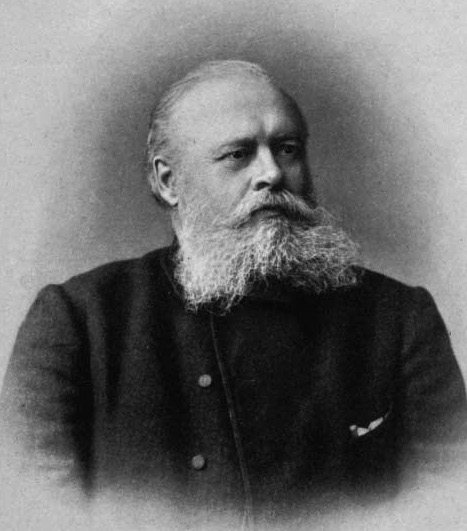
\includegraphics[width=\linewidth]{images/book2/markovnikov.jpg}
\end{minipage}\hfill
\begin{minipage}[t]{0.76\linewidth}\vspace{0pt}
Vladimir Markovnikov menyatakan aturannya pada abad kesembilan belas, dari
produk-produk yang diamatinya bersama kimiawan lain, jauh sebelum
\omterm{def:b1:electronic-effects:intermediates}{karbokation} atau \omterm{def:b1:electronic-effects:curly-arrow}{panah lengkung} dikenal: sebuah keteraturan alam yang
dituliskan sebelum dapat dijelaskan. Pernyataan modernnya melalui
kestabilan \omterm{def:b1:electronic-effects:intermediates}{karbokation} memperlihatkan apa yang ditambahkan sebuah
mekanisme pada aturan empiris: mekanisme itu mengatakan kapan aturan itu
seharusnya gagal. (Potret dari sebuah obituari yang terbit pada tahun
1905, domain publik, Wikimedia Commons.)
\end{minipage}
\end{history}

\section{Latihan}

\begin{exercise}[$\star$]\label{exo:b1:electrophilic-additions:1}
Tentukan produk utama dari: propena + HCl; 2-metilpropena + HBr;
1-metilsikloheksena + HBr; but-2-una + satu ekuivalen HCl.
\end{exercise}

\begin{exercise}[$\star$]\label{exo:b1:electrophilic-additions:2}
Tuliskan produk brom dengan etena, sikloheksena, dan propena. Berilah
namanya.
\end{exercise}

\begin{exercise}[$\star$]\label{exo:b1:electrophilic-additions:3}
Alkohol manakah yang dihasilkan oleh \omterm{def:b1:electrophilic-additions:hydration}{hidrasi} setiap alkena berikut yang
dikatalisis asam: propena, 2-metilpropena, metilenasikloheksana?
\end{exercise}

\begin{exercise}[$\star$]\label{exo:b1:electrophilic-additions:4}
Senyawa manakah di antara berikut ini yang bereaksi dengan natrium amida:
propuna, but-2-una, propena, etanol? Tuliskan reaksinya.
\end{exercise}

\begin{exercise}[$\star\star$]\label{exo:b1:electrophilic-additions:5}
Tuliskan mekanisme lengkap \omterm{def:b1:electrophilic-additions:hydration}{hidrasi} 2-metilpropena dengan \omterm{def:b1:electronic-effects:curly-arrow}{panah lengkung},
dan jelaskan mengapa reaksi baliknya disukai dalam asam pekat yang panas.
\end{exercise}

\begin{exercise}[$\star\star$]\label{exo:b1:electrophilic-additions:6}
Jelaskan dengan postulat Hammond mengapa 2-metilpropena bereaksi dengan
HCl jauh lebih cepat daripada propena.
\end{exercise}

\begin{exercise}[$\star\star$]\label{exo:b1:electrophilic-additions:7}
Brom bereaksi dengan sikloheksena. Tunjukkan bahwa produknya adalah
\textit{trans}-1,2-dibromosikloheksana, dan nyatakan apakah zat itu \omterm{def:b1:stereochemistry-in-depth:stereocentre}{kiral}
dan apakah produknya aktif optis.
\end{exercise}

\begin{exercise}[$\star\star$]\label{exo:b1:electrophilic-additions:8}
Usulkan mekanisme adisi HCl pada 3-metilbut-1-ena yang terutama
menghasilkan 2-kloro-2-metilbutana.
\end{exercise}

\begin{exercise}[$\star\star$]\label{exo:b1:electrophilic-additions:9}
Usulkan sintesis heks-2-una dari propuna dan sebuah haloalkana, dan
sintesis 1-fenilbut-2-un-1-ol dari propuna dan benzaldehida.
\end{exercise}

\begin{exercise}[$\star\star\star$]\label{exo:b1:electrophilic-additions:10}
Buktikan stereokimia adisi brom pada kedua but-2-ena dengan gambar: ion
bromonium, serangan anti pada setiap karbon, \omterm{def:b1:stereochemistry-in-depth:representations}{representasi Cram}
produk-produknya, dan deskriptornya. Hitunglah banyaknya \omterm{def:b1:stereochemistry-in-depth:isomers}{stereoisomer} yang
terbentuk dalam setiap kasus.
\end{exercise}

\begin{exercise}[$\star\star\star$]\label{exo:b1:electrophilic-additions:11}
Air brom dengan propena menghasilkan 1-bromopropan-2-ol sebagai produk
utama. Jelaskan regiokimianya: mengapa air menyerang karbon ion bromonium
yang lebih tersubstitusi?
\end{exercise}

\begin{exercise}[$\star\star\star$]\label{exo:b1:electrophilic-additions:12}
Sebuah hidrokarbon \ce{C5H10} menghilangkan warna air brom dan mengadisi
HBr menghasilkan 2-bromo-2-metilbutana; \omterm{def:b1:electrophilic-additions:hydration}{hidrasinya} menghasilkan
2-metilbutan-2-ol. Temukan dua struktur yang mungkin dan usulkan cara
untuk membedakannya.
\end{exercise}

\section{Soal: Dua Butena dan Brom}

\begin{problem}[{Soal akhir pekan --- kedua but-2-ena, mekanisme bromonium,
dibromida meso dan rasemat, rotasi optisnya, dan massa yang
diperoleh}]
\label{pb:b1:electrophilic-additions:1}
Sebuah laboratorium mempunyai dua botol but-2-ena, yang satu \cip{Z}
murni, yang lain \cip{E} murni, dan mereaksikan \qty{5.60}{g} dari
masing-masing dengan brom dalam diklorometana. Massa molar
(\unit{g/mol}): \ce{C4H8} 56.0, \ce{Br2} 159.8, \ce{C4H8Br2} 215.8.

\medskip
\noindent\textbf{Bagian I --- Kedua alkena.}
\begin{enumerate}
  \item Gambarlah \cip{Z}- dan \cip{E}-but-2-ena dan berikan alasan
        deskriptornya.
  \item Apakah keduanya \omterm{def:b1:stereochemistry-in-depth:isomers}{stereoisomer}? \omterm{def:b1:stereochemistry-in-depth:enantiomers}{Enantiomer} atau \omterm{def:b1:stereochemistry-in-depth:enantiomers}{diastereomer}?
  \item Mengapa keduanya tidak saling berubah pada suhu kamar?
  \item Manakah yang lebih stabil, dan mengapa?
  \item Tuliskan persamaan keseluruhan adisi brom.
  \item Berapa \omterm{def:b1:stereochemistry-in-depth:stereocentre}{pusat stereogenik} yang dimiliki 2,3-dibromobutana? Berapa
        \omterm{def:b1:stereochemistry-in-depth:isomers}{stereoisomer} paling banyak, dan berapa yang sebenarnya?
\end{enumerate}

\medskip
\noindent\textbf{Bagian II --- Mekanismenya.}
\begin{enumerate}[resume]
  \item Tuliskan pembentukan ion bromonium dengan \omterm{def:b1:electronic-effects:curly-arrow}{panah lengkung}.
  \item Mengapa yang terbentuk ion bromonium berjembatan dan bukan
        \omterm{def:b1:electronic-effects:intermediates}{karbokation} terbuka?
  \item Tuliskan pembukaan ion itu oleh bromida.
  \item Mengapa bromida menyerang dari sisi yang berseberangan dengan
        jembatan?
  \item Adisi jenis apakah yang dihasilkan?
  \item Mengapa pelarutnya diklorometana dan bukan air?
\end{enumerate}

\medskip
\noindent\textbf{Bagian III --- Produk-produknya.}
\begin{enumerate}[resume]
  \item Dari \cip{E}-but-2-ena: gambarlah produk serangan pada C2 dan
        tentukan deskriptor C2 dan C3.
  \item Sama halnya untuk serangan pada C3. Bandingkan.
  \item Tunjukkan bahwa produknya meso.
  \item Dari \cip{Z}-but-2-ena: gambarlah kedua produk beserta
        deskriptornya.
  \item Dalam perbandingan berapa keduanya terbentuk? Berilah nama
        campuran itu.
  \item Apakah reaksi ini stereospesifik? Berikan alasannya.
\end{enumerate}

\medskip
\noindent\textbf{Bagian IV --- Rotasi dan massa.}
\begin{enumerate}[resume]
  \item Rotasi optis apakah yang diperlihatkan oleh produk alkena \cip{Z}?
  \item Hitunglah jumlah masing-masing alkena.
  \item Hitunglah massa dibromida yang diharapkan dari masing-masing pada
        \omterm{def:b1:extent-q-and-k:fractional-extent}{rendemen} \qty{85}{\percent}.
  \item Nyatakan \omterm{def:b1:stereochemistry-in-depth:optical-activity}{rotasi spesifik} dibromida yang diperoleh dari
        \cip{E}-but-2-ena, beserta massa yang diperoleh.
\end{enumerate}
\end{problem}
